%%%%%%%%%%%%%%%%%%%%%%%%%%%%%%%%%%%%%%%%%%%%%%%%%%%%%%%%%%%%%%%%%%%%%%%%%%%%
%%%%%%%%%%%%%%%%%%%%%%%%%%%%%%%%%%%%%%%%%%%%%%%%%%%%%%%%%%%%%%%%%%%%%%%%%%%%
%%%%%%%%%%%%%%%%%%%%%%%%% PAQUETES QUE UTILIZO %%%%%%%%%%%%%%%%%%%%%%%%%%%%%
%%%%%%%%%%%%%%%%%%%%%%%%%%%%%%%%%%%%%%%%%%%%%%%%%%%%%%%%%%%%%%%%%%%%%%%%%%%%
%%%%%%%%%%%%%%%%%%%%%%%%%%%%%%%%%%%%%%%%%%%%%%%%%%%%%%%%%%%%%%%%%%%%%%%%%%%%

\documentclass[letter, 11pt, twoside]{report}
\usepackage{amsthm}
\usepackage[many]{tcolorbox}
\usepackage{thmtools}
\usepackage{amssymb,bm,amsfonts,amsmath}
\usepackage[utf8]{inputenc}
\usepackage[spanish]{babel}
\usepackage[export]{adjustbox}
\usepackage{hyperref}
\usepackage{enumerate}
\usepackage{makeidx}
\usepackage{float}
\usepackage{graphicx, import}
\usepackage{subfig}
\usepackage{upgreek}
\usepackage{float}
\usepackage[all]{xy}
\usepackage{thmtools}
\usepackage{titlesec}
\usepackage{mathrsfs}
\usepackage{multicol}
\usepackage{tikz-cd}
\usetikzlibrary{patterns}
\usetikzlibrary{plotmarks}
\usepackage{wrapfig}
\usepackage{stmaryrd}
\usepackage{subfloat}
\usepackage{svg}
\usepackage{yfonts}
\usepackage{fancyhdr}
\usepackage{pifont}
\usepackage{pdfpages}
\usepackage{ marvosym }
\usepackage{hyperref}
\usepackage{pdflscape}
\usepackage{setspace}
\usepackage{color}
\usepackage{bm}
\usepackage{epigraph}
\usepackage{quotchap}
\usepackage[framemethod=TikZ]{mdframed}
\usepackage[nottoc,numbib]{tocbibind}
\usepackage[customcolors]{hf-tikz}
\usetikzlibrary{babel}
% PARA VER LAS REFERENCIAS LABELS
% \usepackage[notcite,color]{showkeys}
% CHECA http://www.tug.dk/FontCatalogue/iwonalightcondensed/
\usepackage[light,math]{iwona}
\usepackage[T1]{fontenc}
\usepackage{MnSymbol}
\usepackage{varwidth} % CAJA DE EJERCICIOS Y \SOMBREADO
\tcbuselibrary{vignette,many}
\tcbuselibrary{skins}
\usepackage{pgfplots}
\usepgfplotslibrary{fillbetween}
\pgfplotsset{compat=1.16}
\usepackage{xcolor}
% PARA ESCRIBIS CÓDIGO Y PSEUDOCÓDIGO
\usepackage{algorithm}
\usepackage{algpseudocode}
\usepackage{listings}
\usepackage{color, xcolor}


%%%%%%%%%%%%%%%%%%%%%%%%%%%%%%%%%%%%%%%%%%%%%%%%%%%%%%%%%%%%%%%%%%%%%%%%%%%%
%%%%%%%%%%%%%%%%%%%%%%%%%%%%%%%%%%%%%%%%%%%%%%%%%%%%%%%%%%%%%%%%%%%%%%%%%%%%
%%%%%%%%%%%%%%%%%%%%%%%%% MEMO PYTHON Y C %%%%%%%%%%%%%%%%%%%%%%%%%%%%%%%%%%
%%%%%%%%%%%%%%%%%%%%%%%%%%%%%%%%%%%%%%%%%%%%%%%%%%%%%%%%%%%%%%%%%%%%%%%%%%%%
%%%%%%%%%%%%%%%%%%%%%%%%%%%%%%%%%%%%%%%%%%%%%%%%%%%%%%%%%%%%%%%%%%%%%%%%%%%%

%CÓMO QUEDERÁ EL COLOREADO Y HIGHLIGHT DEL CÓDIGO
\definecolor{dkgreen}{rgb}{0.9,0.6,0.8}
\definecolor{blue}{rgb}{0.0,0.49,0.4}
\definecolor{gray97}{gray}{.97}
\definecolor{gray75}{gray}{.75}
\definecolor{gray45}{gray}{.45}
\definecolor{codepurple}{rgb}{0.58,0,0.82}
\definecolor{backcolour}{rgb}{0.95,0.95,0.92}
\definecolor{codegreen}{rgb}{0,0.6,0}
\definecolor{codegray}{rgb}{0.5,0.5,0.5}

\lstdefinestyle{mystyle}{
    backgroundcolor=\color{gray97},
    commentstyle=\color{cyan!75!black},
    keywordstyle=\color{magenta},
    numberstyle=\tiny\color{codegray},
    stringstyle=\color{codepurple},
    basicstyle=\ttfamily\footnotesize,
    breakatwhitespace=false,
    breaklines= true,
    captionpos=b,
    keepspaces=true,
    numbers=left,
    numbersep=5pt,
    showspaces=false,
    showstringspaces=false,
    showtabs=false,
    tabsize=2,
    language=bash,   %% PHP, C, Java, etc... bash is the standard
    extendedchars=true,
    inputencoding=latin1
}

\lstset{style=mystyle, literate =
                        {í}{{\'i}}1
                        {á}{{\'a}}1
                        {é}{{\'e}}1
                        {ó}{{\'o}}1
                        {ú}{{\'u}}1
                        {ñ}{{\~n}}1
                        {ü}{{\"u}}1
                            }

%%%%%%%%%%%%%%%%%%%%%%%%%%%%%%%%%%%%%%%%%%%%%%%%%%%%%%%%%%%%%%%%%%%%%%%%%%%%
%%%%%%%%%%%%%%%%%%%%%%%%%%%%%%%%%%%%%%%%%%%%%%%%%%%%%%%%%%%%%%%%%%%%%%%%%%%%
%%%%%%%%%%%%%%% COLORES DEL PAQUETE SHOWKEYS %%%%%%%%%%%%%%%%%%%%%%%%%%%%%%%
%%%%%%%%%%%%%%%%%%%%%%%%%%%%%%%%%%%%%%%%%%%%%%%%%%%%%%%%%%%%%%%%%%%%%%%%%%%%
%%%%%%%%%%%%%%%%%%%%%%%%%%%%%%%%%%%%%%%%%%%%%%%%%%%%%%%%%%%%%%%%%%%%%%%%%%%%

\definecolor{refkey}{rgb}{255,0,0}
\definecolor{labelkey}{rgb}{255,0,0}
\definecolor{mirosa}{HTML}{FF007F}

%%%%%%%%%%%%%%%%%%%%%%%%%%%%%%%%%%%%%%%%%%%%%%%%%%%%%%%%%%%%%%%%%%%%%%%%%%%%
%%%%%%%%%%%%%%%%%%%%%%%%%%%%%%%%%%%%%%%%%%%%%%%%%%%%%%%%%%%%%%%%%%%%%%%%%%%%
%%%%%%%%%%%%%%%% MARGENES, VIENE EN EL MANUAL DE LATEX %%%%%%%%%%%%%%%%%%%%%
%%%%%%%%%%%%%%%% FORMATO ME LO PASO RO %%%%%%%%%%%%%%%%%%%%%%%%%%%%%%%%%%%%%
%%%%%%%%%%%%%%%%%%%%%%%%%%%%%%%%%%%%%%%%%%%%%%%%%%%%%%%%%%%%%%%%%%%%%%%%%%%%
%%%%%%%%%%%%%%%%%%%%%%%%%%%%%%%%%%%%%%%%%%%%%%%%%%%%%%%%%%%%%%%%%%%%%%%%%%%%

\parskip=5pt
\hoffset = 0pt
\headsep = 1.5 cm % estaba en 1.5 cm, lo cambie para el header de la imagen
\oddsidemargin = .5cm
\evensidemargin = .5cm
\textheight = 657pt
\textwidth = 15.6cm
\topmargin = -2 cm
\parindent=0mm

%%%%%%%%%%%%%%%%%%%%%%%%%%%%%%%%%%%%%%%%%%%%%%%%%%%%%%%%%%%%%%%%%%%%%%%%%%%%
%%%%%%%%%%%%%%%%%%%%%%%%%%%%%%%%%%%%%%%%%%%%%%%%%%%%%%%%%%%%%%%%%%%%%%%%%%%%
%%%%%%%%%%%%%%%%%%%%%%%% CREACIÓN DE EJERCICIO %%%%%%%%%%%%%%%%%%%%%%%%%%%%%
%%%%%%%%%%%%%%%%%% MODIFICACIÓN PROOF Y QED %%%%%%%%%%%%%%%%%%%%%%%%%%%%%%%%
%%%%%%%%%%%%%%%%%%%%%%%%%%%%%%%%%%%%%%%%%%%%%%%%%%%%%%%%%%%%%%%%%%%%%%%%%%%%
%%%%%%%%%%%%%%%%%%%%%%%%%%%%%%%%%%%%%%%%%%%%%%%%%%%%%%%%%%%%%%%%%%%%%%%%%%%%

\renewcommand{\qedsymbol}{\tiny{$\blacksquare$}}

\newenvironment{solucion}{\begin{proof}[\textcolor{magenta}{Solución}]}{\end{proof}}

\newtcolorbox[auto counter]{ejercicio}[1][]{
% ESTO ES PARA LA CAJA GENERAL
breakable, % por si cambias de pagina
enhanced, % estilo general
% TITULO MODIFICACIONES
coltitle= black,
colbacktitle= white,
titlerule= 0mm,
colframe = magenta,
fonttitle=\bfseries,
title= Ejercicio~\thetcbcounter,
% CAJA LINEA MODIFICACIONES
boxed title style={
  sharp corners,
  rounded corners=northwest,
  rounded corners=northeast,
  % outer arc=0pt,
  % arc=0pt,
  },
% CONTENIDO MODIFICACIONES
colback = white,
fontupper = \itshape,
coltext =  black,
% MARCO MODIFICACIONES
rightrule=0mm,
toprule=0pt,
bottomrule= 0pt,
leftrule = 4pt
}

%%%%%%%%%%%%%%%%%%%%%%%%%%%%%%%%%%%%%%%%%%%%%%%%%%%%%%%%%%%%%%%%%%%%%%%%%%%%
%%%%%%%%%%%%%%%%%%%%%%%%%%%%%%%%%%%%%%%%%%%%%%%%%%%%%%%%%%%%%%%%%%%%%%%%%%%%
%%%%%%%%% CREE COMANDOS PARA FACILITAR ESCRITURA %%%%%%%%%%%%%%%%%%%%%%%%%%%
%%%%%%%%%%%%%%%%%%%%%%%%%%%%%%%%%%%%%%%%%%%%%%%%%%%%%%%%%%%%%%%%%%%%%%%%%%%%
%%%%%%%%%%%%%%%%%%%%%%%%%%%%%%%%%%%%%%%%%%%%%%%%%%%%%%%%%%%%%%%%%%%%%%%%%%%%

\newcommand{\I}[4]{\displaystyle\int\limits_#1^#2 #3 \,\text{d}#4}
\newcommand{\III}[2]{\displaystyle\int#1 \,\text{d}#2}
\newcommand{\II}[1]{\displaystyle\int#1 \,\text{d$x$}}
\newcommand{\fun}[3]{$#1:#2 \longrightarrow #3$}


%%%%%%%%%%%%%%%%%%%%%%%%%%%%%%%%%%%%%%%%%%%%%%%%%%%%%%%%%%%%%%%%%%%%%%%%%%%%
%%%%%%%%%%%%%%%%%%%%%%%%%%%%%%%%%%%%%%%%%%%%%%%%%%%%%%%%%%%%%%%%%%%%%%%%%%%%
%%%%%%%%%%%%%%%%% MODIFIQUE ALGUNOS COMANDOS %%%%%%%%%%%%%%%%%%%%%%%%%%%%%%%
%%%%%%%%%%%%%%%%%%%%% EL INTERLINEADO %%%%%%%%%%%%%%%%%%%%%%%%%%%%%%%%%%%%%%
%%%%%%%%%%%%%%%%%%%%%%%%%%%%%%%%%%%%%%%%%%%%%%%%%%%%%%%%%%%%%%%%%%%%%%%%%%%%
%%%%%%%%%%%%%%%%%%%%%%%%%%%%%%%%%%%%%%%%%%%%%%%%%%%%%%%%%%%%%%%%%%%%%%%%%%%%

\renewcommand{\baselinestretch}{1}

%%%%%%%%%%%%%%%%%%%%%%%%%%%%%%%%%%%%%%%%%%%%%%%%%%%%%%%%%%%%%%%%%%%%%%%%%%%%
%%%%%%%%%%%%%%%%%%%%%%%%%%%%%%%%%%%%%%%%%%%%%%%%%%%%%%%%%%%%%%%%%%%%%%%%%%%%
%%%%%%%%%%%%%%%%%% COLUMNAS ES AMBIENTE MULTICOLS %%%%%%%%%%%%%%%%%%%%%%%%%%
%%%%%%%%%%%%%%%%%%%%%%%%%%%%%%%%%%%%%%%%%%%%%%%%%%%%%%%%%%%%%%%%%%%%%%%%%%%%
%%%%%%%%%%%%%%%%%%%%%%%%%%%%%%%%%%%%%%%%%%%%%%%%%%%%%%%%%%%%%%%%%%%%%%%%%%%%

\setlength{\columnseprule}{1pt}
\def\columnseprulecolor{\color{darktangerine}}

%%%%%%%%%%%%%%%%%%%%%%%%%%%%%%%%%%%%%%%%%%%%%%%%%%%%%%%%%%%%%%%%%%%%%%%%%%%%
%%%%%%%%%%%%%%%%%%%%%%%%%%%%%%%%%%%%%%%%%%%%%%%%%%%%%%%%%%%%%%%%%%%%%%%%%%%%
%%%%% ESPACIO ENTRE RENGLONES,COLUMNAS MATRIX  Y THICK DE \FCOLORBOX %%%%%%%
%%%%%%%%%%%%%%%%%%%%%%%%%%%%%%%%%%%%%%%%%%%%%%%%%%%%%%%%%%%%%%%%%%%%%%%%%%%%
%%%%%%%%%%%%%%%%%%%%%%%%%%%%%%%%%%%%%%%%%%%%%%%%%%%%%%%%%%%%%%%%%%%%%%%%%%%%

\renewcommand{\arraystretch}{1.2} % for the vertical padding (space)
\setlength{\tabcolsep}{0.2 cm} % for the horizontal padding  (space)
\setlength{\fboxrule}{3pt}

%%%%%%%%%%%%%%%%%%%%%%%%%%%%%%%%%%%%%%%%%%%%%%%%%%%%%%%%%%%%%%%%%%%%%%%%%%%%
%%%%%%%%%%%%%%%%%%%%%%%%%%%%%%%%%%%%%%%%%%%%%%%%%%%%%%%%%%%%%%%%%%%%%%%%%%%%
%%%%%%%%%%%%%%%%%%%%%%%%%%% ESTILO DE LA PÁGINAS %%%%%%%%%%%%%%%%%%%%%%%%%%%
%%%%%%%%%%%%%%%%%%%%%%%%%%%%%%%%%%%%%%%%%%%%%%%%%%%%%%%%%%%%%%%%%%%%%%%%%%%%
%%%%%%%%%%%%%%%%%%%%%%%%%%%%%%%%%%%%%%%%%%%%%%%%%%%%%%%%%%%%%%%%%%%%%%%%%%%%

\pagestyle{fancy}
\fancyhf{}
\fancyhead[RE, RO]{}
\fancyhead[LE, LO]{}
\fancyfoot[CE,CO]{\thepage}
\fancyfoot[RE,RO]{\small{\textsc{Y. Sarahi García González}}}
\fancyfoot[LE,LO]{\small{\textsc{Procesamiento de Lenguaje Natural}}}
\chead{\includegraphics[scale=.3]{/Users/ely/Documents/Plantilla/Figures/waves.pdf}}
\renewcommand{\headrulewidth}{0pt}
\renewcommand{\footrulewidth}{0pt}

%%%%%%%%%%%%%%%%%%%%%%%%%%%%%%%%%%%%%%%%%%%%%%%%%%%%%%%%%%%%%%%%%%%%%%%%%%%%
%%%%%%%%%%%%%%%%%%%%%%%%%%%%%%%%%%%%%%%%%%%%%%%%%%%%%%%%%%%%%%%%%%%%%%%%%%%%
%%%%%%%%%%%%% CAPÍTULOS MISMA PÁGINA %%%%%%%%%%%%%%%%%%%%%%%%%%%%%%%%%%%%%%%
%%%%%%%%%%%%%%%%%%%%%%%%%%%%%%%%%%%%%%%%%%%%%%%%%%%%%%%%%%%%%%%%%%%%%%%%%%%%
%%%%%%%%%%%%%%%%%%%%%%%%%%%%%%%%%%%%%%%%%%%%%%%%%%%%%%%%%%%%%%%%%%%%%%%%%%%%

\usepackage{etoolbox}
\makeatletter
\patchcmd{\chapter}{\if@openright\cleardoublepage\else\clearpage\fi}{}{}{}
\makeatother

%%%%%%%%%%%%%%%%%%%%%%%%%%%%%%%%%%%%%%%%%%%%%%%%%%%%%%%%%%%%%%%%%%%%%%%%%%%%
%%%%%%%%%%%%%%%%%%%%%%%%%%%%%%%%%%%%%%%%%%%%%%%%%%%%%%%%%%%%%%%%%%%%%%%%%%%%
%%%%%%%%%%%%%%%%%%%%%%%%%%%%% EMPEZAMOS %%%%%%%%%%%%%%%%%%%%%%%%%%%%%%%%%%%%
%%%%%%%%%%%%%%%%%%%%%%%%%%%%%%%%%%%%%%%%%%%%%%%%%%%%%%%%%%%%%%%%%%%%%%%%%%%%
%%%%%%%%%%%%%%%%%%%%%%%%%%%%%%%%%%%%%%%%%%%%%%%%%%%%%%%%%%%%%%%%%%%%%%%%%%%%

\begin{document}
\synctex=1 % PARA SINCRONIZAR PDF AL PRESIONAR
%%%%%%%%%%%%%%%%%%%%%%%%%%%%%%%%%%%%%%%%%%%%%%%%%%%%%%%%%%%%%%%%%%%%%%%%%%%%
% \begin{savequote}[45mm]
% ---Frase---
% \qauthor{Guillermo Gachuz Atitlán}
% \end{savequote}
%%%%%%%%%%%%%%%%%%%%%%%%%%%%%%%%%%%%%%%%%%%%%%%%%%%%%%%%%%%%%%%%%%%%%%%%%%%%
%%%%%%%%%%%%%%%%%%%%%%%%%%%%%%%%%%%%%%%%%%%%%%%%%%%%%%%%%%%%%%%%%%%%%%%%%%%%
\chapter*{\begin{tabular}{p{12cm}  c}
   \begin{flushright}
    Tarea 6: Embeddings and CNNs\\\small{Y. Sarahi Grcía González}
   \end{flushright} & \includegraphics[scale=0.3, raise =-2cm]{/Users/ely/Documents/Plantilla/Figures/cimat.png} \\
  \end{tabular} }
\vspace{-2cm}
%%%%%%%%%%%%%%%%%%%%%%%%%%%%%%%%%%%%%%%%%%%%%%%%%%%%%%%%%%%%%%%%%%%%%%%%%%%%
%%%%%%%%%%%%%%%%%%%%%%%%%%%%%%%%%%%%%%%%%%%%%%%%%%%%%%%%%%%%%%%%%%%%%%%%%%%


%%%%%%%%%%%%%%%%%%%%%%%%%%%%%%%%%%%%%%%%%%%%%%%%%%%%%%%%%%%%%%%%%%%%%%%%%%%%
%%%%%%%%%%%%%%%%%%%%%%%%%%%%%%%%%%%%%%%%%%%%%%%%%%%%%%%%%%%%%%%%%%%%%%%%%%%%
%%%%%%%%%%%%%%%%%%%%%%%%%%%%%%%%%%%%%%%%%%%%%%%%%%%%%%%%%%%%%%%%%%%%%%%%%%%%
%%%%%%%%%%%%%%%%%%%%%%%%%%%%%%%%%%%%%%%%%%%%%%%%%%%%%%%%%%%%%%%%%%%%%%%%%%%%
%%%%%%%%%%%%%%%%%%%%%%%%%%%%%%%%%%%%%%%%%%%%%%%%%%%%%%%%%%%%%%%%%%%%%%%%%%%%
\section*{Word2Vec}
\begin{itemize}
    \item Explique la estrategia de selección de paralabras dentro de la ventana de contexto en w2v, ¿Por qué se hace así y cuál es la intuición?\\
    El paper presentanta dos Arquitecturas \ref{cbowyskipgram} de red neuronal. Éstas consisten de una capa de entrda, una de proyección y una de salida. La estrategia de selección para ventana de contexto es la misma en ambos casos pero la probabilidad que se busca encontrar depende de cuál de los dos modelos se esté implementando.
    \begin{figure}[H]
      \begin{center}
        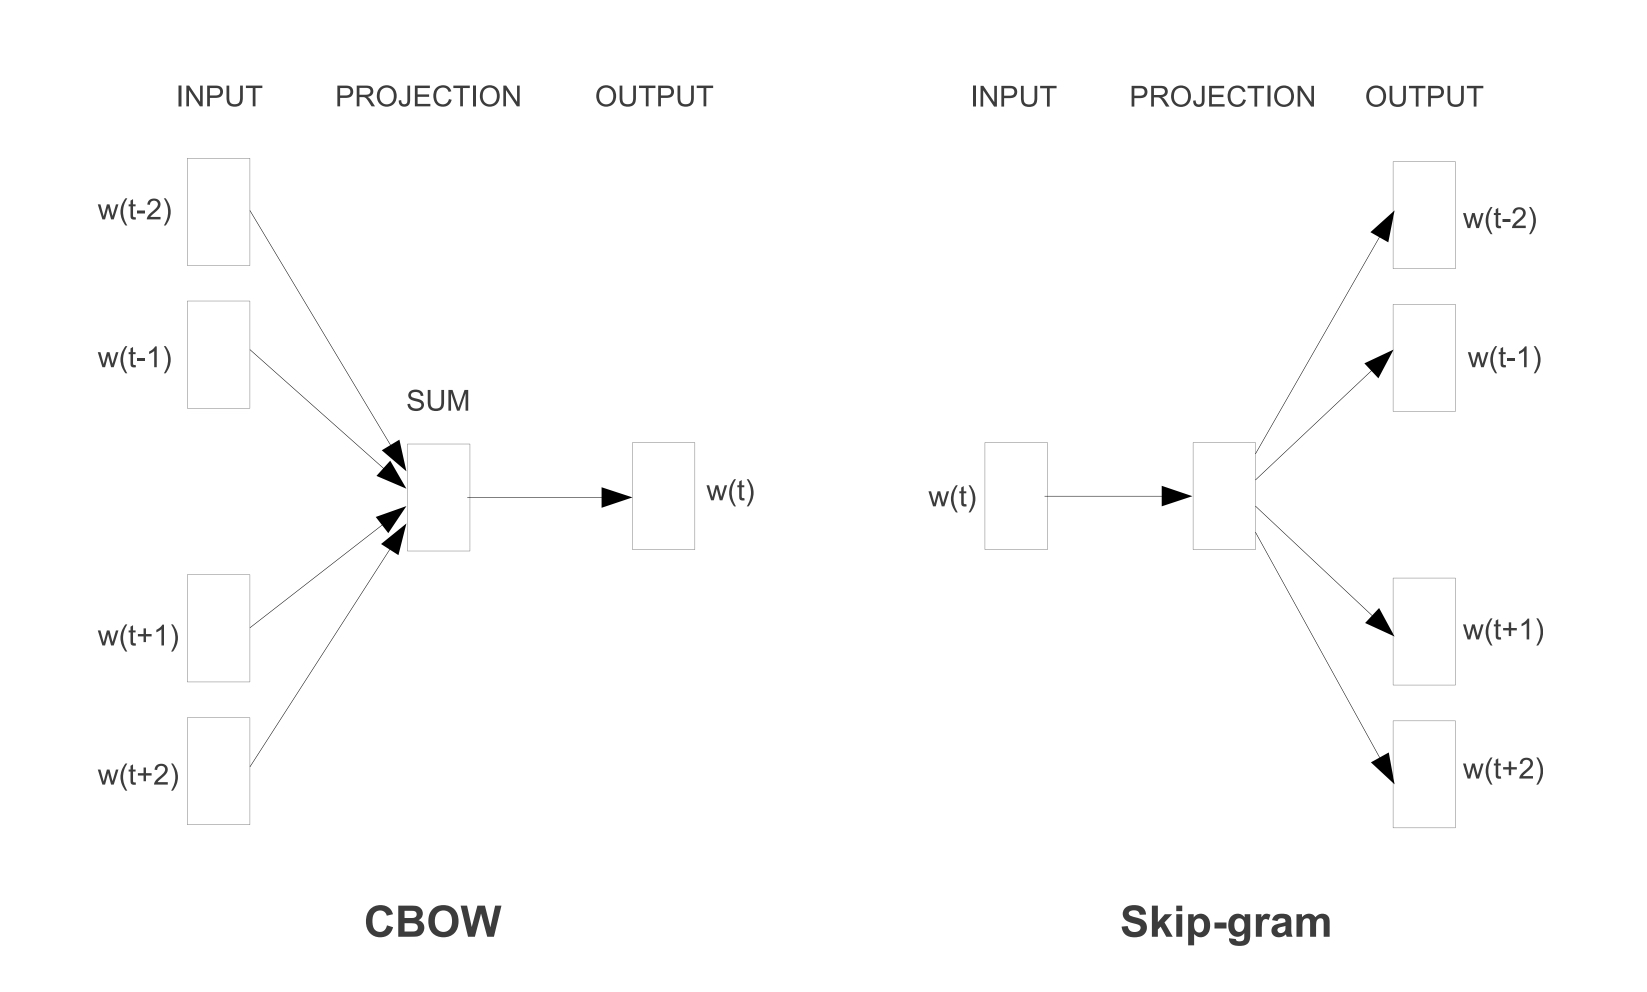
\includegraphics[scale=0.15]{models.jpeg}
        \caption{Arquitecturas propuestas en el paper: CBOW y Skip-gram}
        \label{cbowyskipgram}
      \end{center}
    \end{figure}
    
    Se recorre cada posición en el texto, llamémosle $t$ a la posición actual. Para esta posición $t$, la palabra $w(t)$ es la palabra central y, el contexto son dos palabras a la izquierda (posición $t-2$) y dos palabras a la derecha (posición $t+2$) como se muestra \ref{context}.
    \begin{figure}[H]
      \begin{center}
        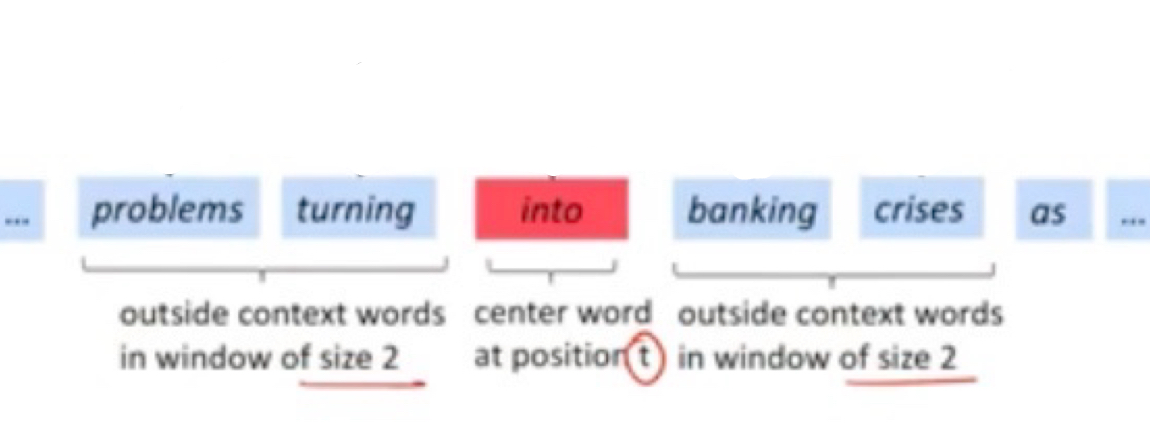
\includegraphics[scale=0.18]{Lenguaje_clase14_word2vec.jpeg}
        \caption{Ventana de contexto de tamaño dos. Palabra central en rojo y palabras \textit{outside context} en azul.}
        \label{context}
      \end{center}
    \end{figure}

    En el caso de que la posición $t$ sea la primera o ultima del documento, se agregan los tokens especiales de inicio/final de oración. 

    Cómo se puede ver en el diagrama \ref{cbowyskipgram}, la ventana de contexto se utiliza de distinta forma en cada una de las aruitecturas. En el caso de CBOW, a partir de las palbras \textit{outside} se calcula la probabilidad para palabra central dado el contexto que la rodea $P(w_t|w_{t-i})$ con $i\in\{-2,-1,1,2\}$. En el caso de Skipgram, se calcula la probabilidad de las palabras del contexto, dada la palabra central de éste contexto. 

    La intuición de esto sigue siendo la senántica distribucional: las palabras que se usan y aparecen en los mismos contextos tienden a transmitir significados parecidos.



    \item ¿Qué estrategia se usa para construir frases de palabras y construir un solo vector para conceptos basados en más de un token?\\
    Para aprender la representación de un sólo vector para una frase se siguen varios pasos, primero:
    \begin{enumerate}
      \item Se encuentran las palabras que frecuentemente aparecen juntas como una frase.
      \item Se define un score \ref{score} y un cierto umbral, de modo que todos los bigramas por encima de ese umbral se considerarán un único token.
      \begin{equation}
        score(w_i,w_j)=\frac{count(w_i,w_j)-\delta}{count(w_i)*count(w_j)}
        \label{score}
      \end{equation}
      \item Estas frases se reemplazan por un único token (en lugar los $n$ que conformn la frase) en el dataset de entrenamiento. 
    \end{enumerate}


    Notemos que sólo las paralabras que aparecen juntas en uno (o unos pocos) cotexto específico serán tomadas en cuenta como un token, de modo que \textit{Estado de México} sería uno de éstos ejemplos, pero \textit{esto es} no lo sería. Pues las pabras \textit{esto} y \textit{es} podrían aparecer juntas en cualquier texto del español, mientras que, a menos que estemos hablando del estado específico, \textit{estado}, \textit{de} y \textit{México} no co-ocurren. 

  
    \item Según el autor de w2v ¿cuáles podrían ser las ventajas/desventajas de CBOW y Skipgram?
    En el primer paper (Efficient Estimation of Word Representations in vector space) se mencionan éstas dos arquitecturas y algunas otras en la sección dos \textit{Model Architectures} y en los resultados. 
    
    De la sección dos se puede resumir que la ventaja de los modelos propuestos por el paper tienen que ver con la complejidad. La complejidad la definen como el número de parámetros a los que se necista acceder para enterenar completamente el modelo. Y precisamente uno de los objetivos del paper es maximizar el accuracy y al mismo tiempo disminuir la complejidad computacional en sus modelos.

    En los resultados se menciona que la evaluación se hizo a través de una serie de tareas específicas, tales cómo el preguntare ¿Cuál es la palabra que es similar a "small" en el mismo sentido que "biggest" es similar a "big"?. Se muestran cinco tipos de preguntas semánticas y nueve de preguntas sintácticas, aunque se menciona, en total fueron 8869 semánticas y 10675 sintácticas. Para considerar una respuesta como correcta, el resultado de las operaciones algebráicas sobre los vectores debe de ser el \textbf{más cercano}  a la palabra correcta. 

    \begin{figure}[H]
      \begin{center}
        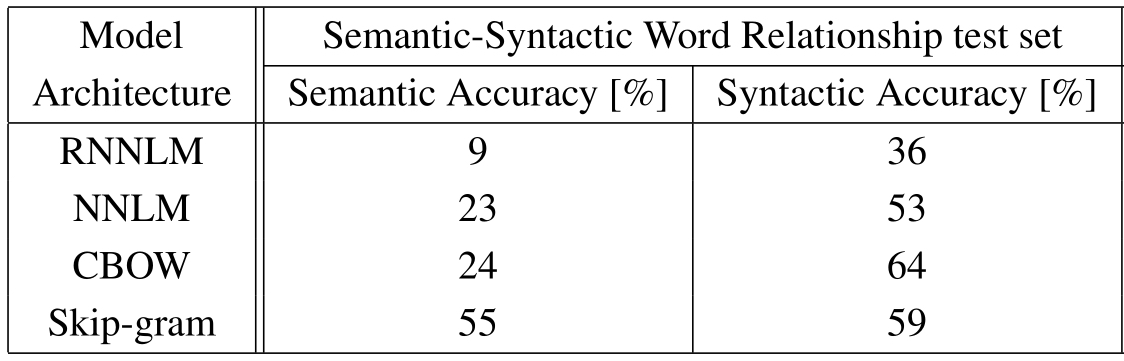
\includegraphics[scale=0.25]{tabla1.jpeg}
        \caption{Tabla comparativa de arquitecturas usando modelos entrenados sobre los mismos datos. Vectores de dimensión 640.}
        \label{models}
      \end{center}
    \end{figure}
    
   En la tabla \ref{models} del paper w2va-1 se observa que los modelos propuesto en éste superan a las aruitecturas RNNLM y NNLM en ambas tipos de preguntas. Entre CBOW y Skipgram, el primero es mejor en la cuestión sintáctica y el segundo el la semántica (dos veces mejor). Sin mecionar, como ya se dijo antes que estas aruitecturas tiene una complejidad mucho menor.

   Se mencionan dos comparaciones más bajo distintas codiciones y los resultados son similares. CBOW es mejor que NNLM  y que Skip-gram en la parte sintáctica. Skip-gram es  mejor que NNLM en esta tarea y es mucho mejor que todos los modelos en la parte semántica.

   Las ventajas entonces se resumen en ser computacionalmente menos complejas (con la complejidad definida en el paper), además de mostrar mejor accuracy (medida con las tareas propuestas en el paper). Particularmente Skip-gram es muy superior (a CBOW y los demás modelos) en la tarea semántica.

   Una desventaja que se menciona es que para poder entrenar grandes cantidades de datos, e quita la capa oculta del modelo lo que tiene omo consecuencia un modelo menos preciso, sin embargo esto se compensa precisamente con el ser más eficiente con grandes cantidades de texto. De modo que estos modelos NO son convenientes si no se cuenta con mucho texto.

    \item ¿Cuáles son las diferencias entre usar Hierarchical Softmax, Negative Sampling y NCE? ¿Cuál recomienda el autor y por qué?
    
    En el modelo de Skipgram, dada la secuencia de palabras $w_1$, $w_2$, $w_T$, el objetivo de éste es maximizar el promedio de la log-verosimilitud dado por

    \begin{eqnarray}
      \frac{1}{T}\sum_{t=1}^{T}\sum_{-c\leq j \leq c}log (p(w_{t+j}|w_t))
    \end{eqnarray}
     Con $c$ el tamaño de la ventana de contexto. Aquí lo interesante es encontrar la probabilidad $p(w_{t+j}|w_t)$. Una manera de calcularla es con la función \textbf{softmax} \ref{softmax}, pero es impráctico debido a que de ésta, el costo computaciónal es proporcional al tamaño del vocabulario.
     \begin{eqnarray}
      p(w_{O}|w_I)=\frac{exp(w_o * w_i )}{\sum_{w\in W}exp(w * w_i )}
      \label{softmax}
    \end{eqnarray}

     Para resolver este inconveniente se usan distintas aproximaciones para calcular la probabilidad de interés, entre ellas Hierarchical Softmax (HS), Negative Sampling (NS) y Noise Contrastive Estimation (NCE). A continuación discutiremos cada una de ellas.



    \begin{enumerate}
      \item Hierarchical Softmax
      
      La principal ventaja sobre Softmax es que en lugar de evaluar sobre todo el vocabulario $W$, sólo se evaluan $log_2(W)$ nodos en la red neuronal. Representa la capa de salida como un arbol binario con W palabras como sus hijas y cada nodo es la probabilidad relativa de sus nodos hijo.
      Así, se puede llegar a cada palabra $w$ por un camino desde la raíz del árbol. Sea $n(w, j)$ el j-ésimo nodo en el camino desde la raíz hasta w, y sea $L(w)$ la longitud de este camino, entonces $n(w, 1) = raiz$ y $n(w, L(w)) = w$. Además, para cualquier nodo interno n, sea $ch(n)$ un hijo fijo arbitrario de $n$, entonces, la softmax jerárquica define $p(w_O|w_I )$ de la siguiente manera:

      \begin{equation}
        p(w|wI ) = \prod_{j=1}^{L(w)-1} \sigma \left( \left[ \left[ n(w, j + 1) = ch(n(w, j)) \right] \right] \cdot v_{n(w,j)}^\prime v_{wI} \right)
      \end{equation}

      
      
      \item Noise Contrastive Estimation 
      

      La idea básica es convertir el problema de estimar una probabilidad de palabra en un problema de clasificación binaria, lo que lo hace más manejable y eficiente computacionalmente. En lugar de tratar de calcular la probabilidad de que una palabra sea la correcta, se utiliza el enfoque de "contraste de ruido" donde el modelo se entrena para distinguir entre datos reales y datos generados artificialmente.
  
      NCE maximiza la probabilidad logarítmica de la softmax \ref{softmax} y busca poder diferenciar entre datos y \textit{ruido} mediante regresión logística. Sin embaergo, Skip-gram sólo se preocupa por aprender representaciones vectoriales de alta calidad, de manera que podemos simplificar siempre y cuando las representaciones vectoriales conserven su calidad. 


      El ruido se genera
      \item Negative Sampling
      Negative Sampling define como aproximación a la log-probabilidad de enteres a la ecuación \ref{NS}. La tarea consiste en distinguir la palabra objetivo de las selecciones de la distribución de ruido 
      \begin{equation}
        \text{log} \sigma(v'^\top_{w_O} v_{w_I}) + \sum_{i=1}^{k} \mathbb{E}_{w_i \sim P_n(w)} \left[ \text{log} \sigma(-v'^\top_{w_i} v_{w_I}) \right]
        \label{NS}
      \end{equation}
      
    La idea es eligir un subconjunto pequeño y aleatorio de palabras no vecinas (negativas) de la palabra objetivo $w_o$. Estas palabras negativas se muestrean de acuerdo con alguna distribución de probabilidad, como la distribución unigram, donde las palabras más frecuentes tienen más probabilidades de ser seleccionadas como ejemplos negativos.
    \end{enumerate}

    El autor recomienda Negative Sampling (la aproximación que propone el paper) para palabras muy comunes. Además se encontraron buenos resultados usando el subsampling de palabras más frecuentes pues hace los entrenamientos más rápidos y hay una mejor representación de las palabras raras.

    \item ¿Cuál diría usted que es la principal conclusión y aportación del paper de w2v? ¿Qué crítica hría usted a estos papers de w2v?
    
    Del primer paper, para mí la principal conclusión es que se pueden obtener vectores de representación de palabras de muy buena calidad empleando un modelo muy sencillo (siempre y cuando se tenga mucho texto). 

    Y del segundo paper, creo que fue mostrar que las representaciones vectoriales de las palabras muestran una estructura linealque permite hacer razonamientos de tipo analogía. 
    En este paper también se mencionó que pudieron entrenar el modelo en una cantidad de texto con muchos más ordenes de margnitud debido a lo simple de la arquitectura lo que va de la mano con la conclusión anterior.
\end{itemize}


%%%%%%%%%%%%%%%%%%%%%%%%%%%%%%%%%%%%%%%%%%%%%%%%%%%%%%%%%%%%%%%%%%%%%%%%%%%%
%%%%%%%%%%%%%%%%%%%%%%%%%%%%%%%%%%%%%%%%%%%%%%%%%%%%%%%%%%%%%%%%%%%%%%%%%%%%
%%%%%%%%%%%%%%%%%%%%%%%%%%%%%%%%%%%%%%%%%%%%%%%%%%%%%%%%%%%%%%%%%%%%%%%%%%%%
%%%%%%%%%%%%%%%%%%%%%%%%%%%%%%%%%%%%%%%%%%%%%%%%%%%%%%%%%%%%%%%%%%%%%%%%%%%%
%%%%%%%%%%%%%%%%%%%%%%%%%%%%%%%%%%%%%%%%%%%%%%%%%%%%%%%%%%%%%%%%%%%%%%%%%%%%


\section*{Glove}

\begin{itemize}
  \item ¿Qué desventaja trata de solucionar de W2V?
  
  Lo primero que se menciona es que word2vec no utiiza adecuadamente la parte estadística del del corpus con que entrena pues se entrena en contextos locales separados que escanean todo el texto en lugar de tomar en cuenta la co-ocurrencia global de las palabras. 
  Además a lo largo del texto menciona un par de veces que, si bien las estadísticas obtenidas de la co-ocurrencia de palabras, en w2v no es claro este hecho. 

  \item Describa con sus propias palabras cuál es la principal estrategia para lograrlo.
  
  Para empezar, el nombre nos da una idea, GloVe representa Global Vectors, pues se busca capturar las estadísticas globales del texto con este modelo (a diferencia de w2v).

  Una de las ideas básicas para lograr esto es no utilizar directamente la probabilidad de co-ocurrencia $P_{i,j}$ (probabilidad de que el término j co-ocurra con el término i), sino la relación de la probabilidad de co-ocurrencia con otros términos $k$:  $$\frac{P_{i,k}}{P_{j,k}}$$
  Usando esta relación, si el término k está muy relacionado con j pero no con i, el resultado será grande, y viceversa, si está muy relacionado con i pero no con j, el resultado será pequeño y cuando k esté muy relacionado o no de ambas pabras, será cercano a 1.

  Así, esta relación entre probabilidades nos da una nueva caracterización de las co-ocurrencias entre dos palabras que considera la parte local y global. 

  Y de lo anterior se desprende el método propuesto, pues se plantea un modelo que, junto con las propiedades que se deben de cumplir por la naturaleza del problema y tomando en cuenta que las ocurrencias frecuencias sólo añaden ruido al problema se construye la función de costo:

  \begin{equation}
    J = \sum_{i=1}^{V} \sum_{j=1}^{V} f(X_{ij}) \left( w_i^T \tilde{w}_j + b_i + \tilde{b}_j - \text{log}(X_{ij}) \right)^2
    \end{equation}

    Donde V es el tamaño de vocabulario, $X_{ij}$ es el numero de veces que co-ocurren los términos $i$ y $j$, y $f$ una función que cumple ser cero en cero, ser no decresiente y hacerse pequeña cuando x es grande. De este modo, da menor importancia a las  co-ocurrencias más frecuentes.

    Llega a esta misma ecuación desde el enfoque de w2v también donde hace explícito el otro fallo que tiene dicho modelo (el no ser transparente con el hecho de que se utilizan estadísiticas de co-ocurrencia).
    
  \item Explique las principales conclusiones de los experimentos. Comente si cree que se logró el objetivos.
  
  Se comentan tres distintos experimentos realizados para evaluar el modelo: Word Analogies, Word Similarity, y Named entity recognition.
  
  El primero, según el paper, es el de mayor interés debido a que se busca encontrar una estructura vectorial adecuada. 
  Como puede observarse en la siguiente tabla, GloVe mejora en casi todos los casos a los modelos propuestos en w2v aunque no por demasiado comparándolo con Skip-gram (resaltado en color naranja). 


  Se encierra en rosa el Size de los conjuntos del último bloque porue es donde GloVe señala la mayor diferencia en accuracy, sin embargo el tamaño de dataset es 7 veces más grande que SG.


  \begin{figure}[H]
    \begin{center}
      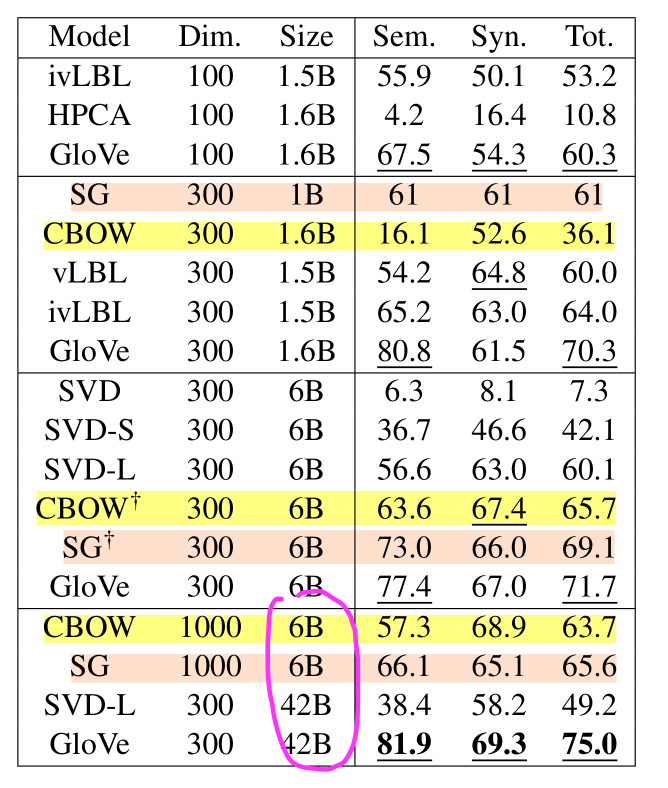
\includegraphics[scale=0.25]{analogy.jpg}
      \caption{Tabla comparativa de modelos en tareas de tipo analogía para distintas dimensiones y tamaños de datasets.}
      \label{an}
    \end{center}
  \end{figure}



  En el segundo experimento, como se muestra en \ref{sim}, GloVe también supera a los demás modelos y del tercer experimento no se menciona nada concreto. 

  \begin{figure}[H]
    \begin{center}
      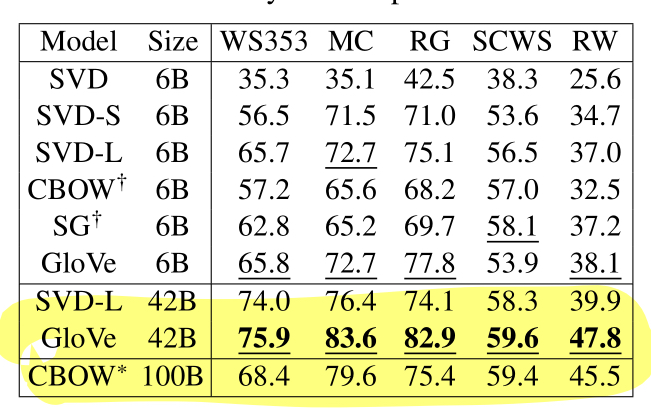
\includegraphics[scale=0.25]{similarity.jpg}
      \caption{Tabla comparativa de modelos en tareas de tipo similitud de palagras para distintas dimensiones y tamaños de datasets.}
      \label{sim}
    \end{center}
  \end{figure}

  Se menciona también que rendimiento es mejor en la parte sintáctica para ventanas de contexto pequeñas y asimétricas, lo cual concuerda con la intuición de que la información sintáctica se extrae principalmente del contexto inmediato y puede depender fuertemente del orden de las palabras. Por otro lado, la información semántica es no local, y se captura mejor con tamaños de ventana más grandes.


  Para el mismo corpus, vocabulario, tamaño de ventana y tiempo de entrenamiento, GloVe supera a word2vec auqnue como el mismo paper menciona, hay muchas variables que pueden modificarse en w2v y tienen un imparcto significativo que no se tomaron en cuenta en este estudio. 

  

  \item ¿Encuentra alguna relación entre Glove y las clásicas TCOR y DOR? ¿Cuáles?
  

  Sí, pues el modelo el modelo se entrena en matrices de co-ocurrencia word-word.
  Además en la función de costo se toma en cuenta una función de pesado que indica la importancia que tiene la co-ocurrencia de las palabras. A aquellas que co-ocurren con demasiada frecuencia con otras palabras se les da un menor peso, pues son palabras comunes y no ayudan verdaderamente a definir otra palabra. Esto es análogo al pesado TFiDF.
  


  \item Principal conclusión y aortación del paper de Glove. ¿Qué crítica haría usted a este paper?
  

  Creo que la principal conclusión del paper es que 
  las representaciones vectoriales de palabras construidas a partir de conteo de ocurrencias y las construidas con base en prediccióin no son dramáticamente diferentes a un nivel fundamental, ya que ambos investigan las estadísticas de co-ocurrencia subyacentes del corpus, pero la eficiencia con la que los métodos basados en conteo capturan estadísticas globales puede ser ventajosa. Y eso es justamente lo que busca ser GloVe: un modelo que utiliza este beneficio de los datos de conteo mientras captura las subestructuras lineales significativas (como en los métodos de predicción).

  Algo que le criticaría es que habla demasiado sobre w2v sin dar información relevante sobre cuál es la estrucutra de ese modelo. Tampoco es claro en como es el entrenamiento de su propio modelo, asumo que es análogo al de w2v pero no lo menciona.

\end{itemize}

%%%%%%%%%%%%%%%%%%%%%%%%%%%%%%%%%%%%%%%%%%%%%%%%%%%%%%%%%%%%%%%%%%%%%%%%%%%%
%%%%%%%%%%%%%%%%%%%%%%%%%%%%%%%%%%%%%%%%%%%%%%%%%%%%%%%%%%%%%%%%%%%%%%%%%%%%
%%%%%%%%%%%%%%%%%%%%%%%%%%%%%%%%%%%%%%%%%%%%%%%%%%%%%%%%%%%%%%%%%%%%%%%%%%%%
%%%%%%%%%%%%%%%%%%%%%%%%%%%%%%%%%%%%%%%%%%%%%%%%%%%%%%%%%%%%%%%%%%%%%%%%%%%%
%%%%%%%%%%%%%%%%%%%%%%%%%%%%%%%%%%%%%%%%%%%%%%%%%%%%%%%%%%%%%%%%%%%%%%%%%%%%


\section*{Otros Papers}
\begin{itemize}
  \item ¿Qué desventaja trata de soluciona FastText?
  

  Una de las imitaciones de w2v es que trataa a  cada palabra como un vector distinto y no considera la estructura interna de las palabras, lo que es una limitación importante para idiomas con una morfología rica, como el español.
  Algunos idiomas contienen muchas formas de palabras que ocurren raramente (o incluso nunca) en el corpus de entrenamiento, lo que dificulta aprender representaciones adecuadas para las palabras.

  En el paper proponen que es posible mejorar las representaciones vectoriales para idiomas morfológicamente ricos utilizando información a nivel de caracteres. La propuesta de FastText es aprender representaciones para n-gramas de caracteres y representar las palabras como la suma de estos vectores. De esta forma, el modelo que se propone tiene en cuenta la información de subpalabras. 
  Esto se evaluó en nueve idiomas con diferentes morfologías, demostrando los beneficios de utilizar información a nivel de caracteres para mejorar la representación de palabras.

  \item ¿Cuál sería la principal desventaja de FastText sobre w2v?
  
   FastText es computacionalmente más intensivo debido a su enfoque de modelado de subpalabras (pues considera subpalabras además de palabras completas) y esto tiene como consecuencia que el tamaño del vocabulario sea mucho mayor. Esto implica más cálculos durante el entrenamiento y el consumo de más recursos computacionales, especialmente en corpus de texto grandes.

   Además, el modelo FastText generalmente requiere más tiempo para entrenar en comparación con Word2Vec debido a la complejidad adicional de considerar subpalabras. En el paper se menciona que utilizando n-gramas de caracteres, es aproximadamente 1.5 veces más lento de entrenar que el baseline skipgram y que procesa alrededor de 105k palabras por segundo por hilo de ejecución, en comparación con las 145k palabras por segundo por hilo de ejecución de Skipgram.

   Sin embargo, creo que a pesar de estas desventajas en términos de rendimiento computacional, FastText ofrece mejoras en la calidad de las representaciones de palabras como se puede apreciar en los resultados del paper, especialmente en idiomas con una morfología rica o en tareas que involucran palabras raras o fuera del vocabulario predefinido.

  \item ¿Qué desventajas trata de solucionar Directional w2v y cómo lo logra? Describa las conclusiones de la sección experimental
  
  \textbf{Desventajas}

  De acuerdo con el paper, skip-gram tiene varias limitaciones, tales como ignorar el orden y las posiciones de las palabras.
  Y este contexto, se presenta el modelo Directional Skip-Gram (DSG), que aborda estas limitaciones al tener en cuenta la orientación de las palabras en el contexto para aprender embeddings de mayor calidad y menor complejidad.

  Para lograr esto, DSG introduce vectores direccionales que representan la orientación de las palabras respecto a la palabra objetivo. Esto permiten al modelo capturar las relaciones semánticas y sintácticas que dependen del orden y la posición de las palabras en el contexto.

  \textbf{Experimentos}

  Se evaluó rapidez de entrenamiento, word similarity y Part-of Speech Tagging, se entrenó con la wikipedia con dos billones de tokens de palabras y se comparó contra el modelo SG original, con el Structured Skip-Gram (SSG) y con una versión simplicicada de éste último (SSSG) que se propuso en el mismo paper.

  Velocidad: Comparado con el modelo original, el modelo SSG muestra una caída relativamente grande al aumentar la ventana de contexto, y una caída mucho menor para el modelo DSG. Al ampliar la ventana de contexto, la brecha de velocidad entre el modelo SSG y SG se hace más grande mientras que la brecha entre DSG y SG se hace más pequeña.

  Word similarity: DSG supera a todos los modelos en corpus pequeños y en corpus grandes, sólo en un dataset queda por debajo pero por muy poco como se puede puede observar en \ref{dsg}:


  \begin{figure}[H]
    \begin{center}
      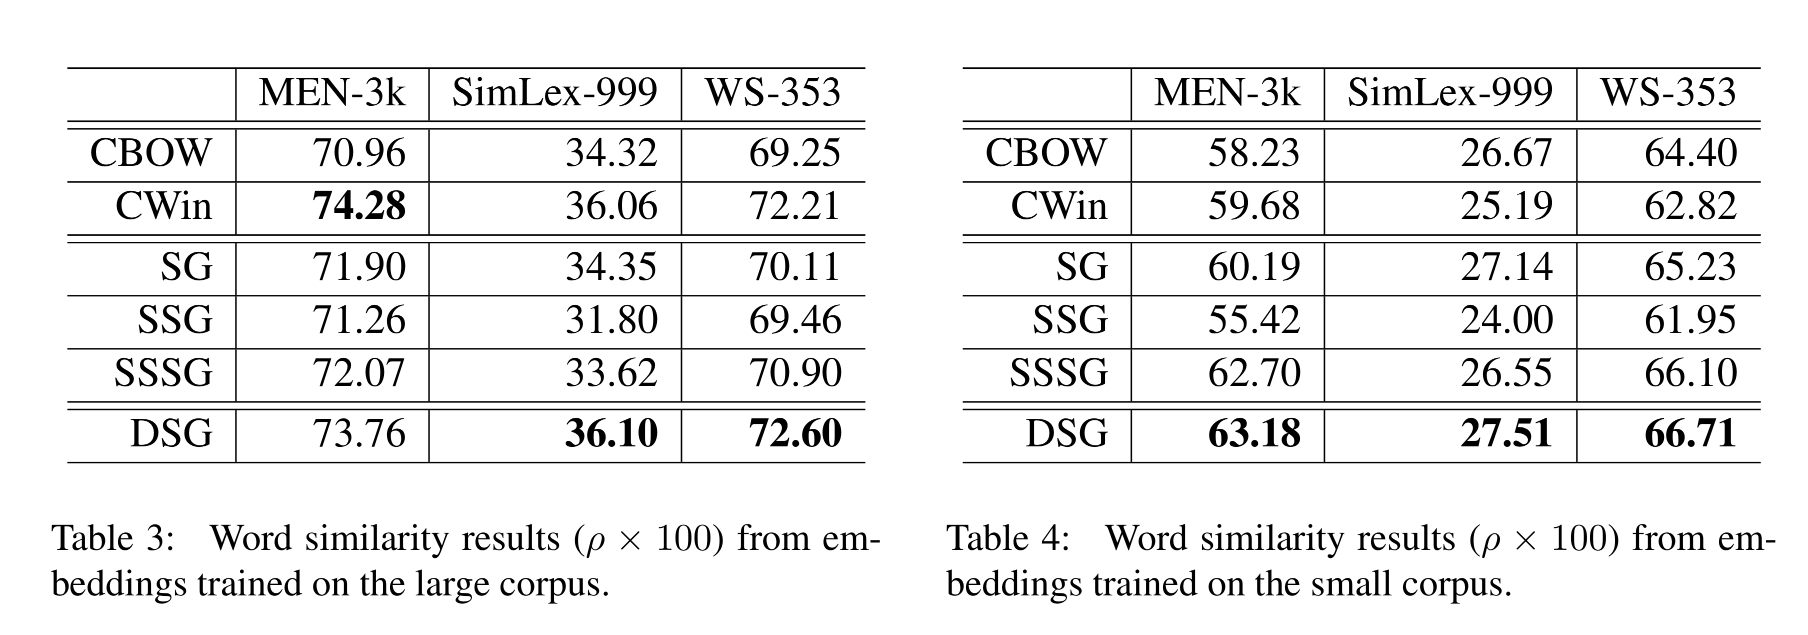
\includegraphics[scale=0.22]{dsg.jpg}
      \caption{Tablas comparativa de modelos en word similarity para corpus grandes y pequeñs.}
      \label{dsg}
    \end{center}
  \end{figure}

  \item ¿Qué se dice a cerca del análisis de complejidad del Dw2v?
  
  Se menciona que se comparó con otros modelos de skip-gram en términos de complejidad espacial y temporal: modelo Structured Skip-Gram (SSG) y el modelo original (SG).

  También se propone un modelo simplificado al SSG, que sería el simplified Structured Skip-Gram (SSSG) donde solo modela el contexto izquierdo y derecho de una palabra dada.
  
  Se señala que el modelo SSG presenta una complejidad notablemente mayor en términos de espacio y tiempo cuando el contexto es más grande. 
  Por otro lado, cada palabra en el modelo DSG solo requiere una operación adicional que la del modelo skip-gram original. Por lo quee si se amplía el contexto, el modelo DSG tendría una velocidad similar.

   La simplificada (SSSG) se presenta como una aproximación del modelo DSG dentro del marco del modelo SSG. En el lado de la salida, SSSG tiene dos vectores "word" respectivamente para el contexto izquierdo y derecho, mientras que DSG tiene un vector "word" y un vector "direction". Como resultado, el vector de dirección de DSG se puede utilizar para predecir explícitamente si el contexto está a la izquierda o a la derecha en la predicción de palabras, mientras que SSSG no lo hace.

  \item ¿En que problemas de clasificación evaluó Kim su CNN?
  \begin{enumerate}
    \item Clasificación de reviews positivas/negativas.
    \item Analisis de sentimiento (etiquetas:muy positivo,positivo, neutral,negativo,muy negativo)
    \item Clasificación de objetivo/subjetivo
    \item Clasificación sobre el tópico de preguntas (etiquetas:persona,lugar,informacón numérica,etc)
  \end{enumerate}
  
  \item En los resultados dónde estuvo involucrado algún método de clasificación con SVM, ¿Cómo fue el resultado respecto a CNNs? ¿Qué features usaba el método basado en SVM?
  
  \item  En sus propias palabras, ¿Qué diferencia tienen las estrategias multi-channel y single-channel?, ¿Cuál recomienda Kim? 
  

  Las arquitecturas de redes neuronales convolucionales (CNN) pueden tener uno o varios canales de entrada, lo que determina cómo se procesan los datos de entrada.


  En la arquitectura multichannel, los canales múltiples pueden representar diferentes fuentes de información, como embbedings y/o características adicionales extraídas del texto. Cada canal puede tener su propio conjunto de filtros, y las salidas de estos canales pueden combinarse de diversas formas antes de pasar a la siguiente capa de la red.

  En el caso del paper de Kim, cada canal es un set de vertores de palbabras, además se especifica que cada filtro se aplica a ambos canales y los resultados se suman para calcular las entradas del \textit{feature map} $\textbf{c}=[c_1,c_2...,c_{n-h+1}]$ donde  $n$ es la longitud de la oración y $h$ el numero de palabras a las que se aplica el filtro. Aunque el filtro se aplica a ambos canales, el backpropagation se hace sólo sobre uno de los dos canales. 

  En el paper se recomienda usar sólo un canal pero con dimensiones extra que puedan modificarse durante el entrenamiento.

  \item ¿Cuál diría usted que es la principal conclusión y aportación
   del paper de Kim? 

   Creo que la principal conclusión es que usando una arquitectura relativamente sencilla (CNN-static) se pueden obtener muy buenos resultados que compiten contra otros modelos de deep learning más sofisticados. 

   Algo que no me gusto del paper fueron las conclusiones, no dicen casi nada a pesar de que se pueden concluir varias cosas a partir de la sección de resultados y discusión.

\end{itemize}



%%%%%%%%%%%%%%%%%%%%%%%%%%%%%%%%%%%%%%%%%%%%%%%%%%%%%%%%%%%%%%%%%%%%%%%%%%%%
%%%%%%%%%%%%%%%%%%%%%%%%%%%%%%%%%%%%%%%%%%%%%%%%%%%%%%%%%%%%%%%%%%%%%%%%%%%%
%%%%%%%%%%%%%%%%%%%%%%%%%%%%%%%%%%%%%%%%%%%%%%%%%%%%%%%%%%%%%%%%%%%%%%%%%%%%
%%%%%%%%%%%%%%%%%%%%%%%%%%%%%%%%%%%%%%%%%%%%%%%%%%%%%%%%%%%%%%%%%%%%%%%%%%%%
%%%%%%%%%%%%%%%%%%%%%%%%%%%%%%%%%%%%%%%%%%%%%%%%%%%%%%%%%%%%%%%%%%%%%%%%%%%%
\end{document}
